\documentclass[]{sigplanconf}
\usepackage{stmaryrd}
\usepackage{listings}
\usepackage{multirow}
\usepackage{array}
\usepackage{subfig}
\usepackage{algorithmic}
\usepackage{algorithm}
\usepackage{amsmath}
\usepackage{xfrac}
%\usepackage{amsthm}
\usepackage{amssymb}
\usepackage{xspace}
%\usepackage[pdftex]{graphicx}
\usepackage{graphicx}
\usepackage{siunitx}
\usepackage[svgnames,table]{xcolor}
\usepackage{natbib}
\usepackage{adjustbox}
\usepackage{tabularx}
\usepackage{booktabs}
\usepackage{placeins}
\usepackage{hyperref}
\hypersetup{
    colorlinks,
	linkcolor={blue!50!black},
	citecolor={blue!50!black},
	urlcolor={blue!80!black}
}
\urlstyle{same}

\newcommand\comment[1]{\ding{110}\ding{43}\textcolor{red}{#1}}

%\newcommand\code[1]{\textsf{\small #1}}
%\DeclareCaptionType{copyrightbox}
\newcommand\sius[1]{\num[group-separator = {,}]{#1}\si{\micro\second}}
\newcommand\sims[1]{\num[group-separator = {,}]{#1}\si{\milli\second}}
\newcommand\sins[1]{\num[group-separator = {,}]{#1}\si{\nano\second}}
\newcommand\tuple[1]{\langle #1 \rangle}
\providecommand{\abs}[1]{\lvert#1\rvert}

%\newcommand{\mc}[3]{\multicolumn{#1}{#2}{#3}}

\begin{document}

\title{Mining timed regular expressions from system traces}

\authorinfo{Greta Cutulenco, Yogi Joshi, Apurva Narayan, and Sebastian Fischmeister}
		   {University of Waterloo, ON, Canada}
		   {\{gcutulen, y2joshi, apurva.narayan, sfischme\}@uwaterloo.ca}

\maketitle


\begin{abstract}

TBD (to be done)

\end{abstract}

\section{Introduction}
%% author: GC

Dynamic behavior of a program can be assessed through an examination of events emitted by the program during execution. For the behavior to be correct it must satisfy a set of specified temporal properties. Temporal properties constrain the order of occurrence of the emitted events. Temporal properties also impose timing constraints on event occurrence. Such specifications are of importance for event driven real-time systems - taking too long to react to an emitted event may lead to a fault in the system. Safety critical systems also need to satisfy temporal properties - complete a sequence of operations to avoid a hazardous situation within a fault tolerant time interval.

Since temporal properties are rarely specified for programs and due to the complexity of the formalisms, temporal properties are automatically extracted from traces of program execution. Dynamic specification inference has shown promising results in many areas, including bug detection, test case specification, and program steering ~\cite{evans2}. The properties can be used to ensure that the system does only what is specified and nothing else. They can be used to evaluate testing completeness - all specified properties are exhibited through existing tests. And lastly they can be used to compile a detailed and complete set of system specifications.

The currently available approaches for extracting temporal properties are however insufficient. They do not scale well for interesting properties with a large number of events. They cannot extract properties efficiently from large and complex system traces. They do not support extraction of properties with timing constraints.

In this paper we propose a framework to automatically mine properties that are in the form of timed regular expressions from system traces. Using an abstract structure of the property the framework constructs a finite state machine (FSM) to serve as an acceptor. We encode the concrete properties in a set of matrices. The FSM is used to evaluate the satisfaction of every potential concrete property in the trace. Using a ranking system we infer the strongest concrete properties that describe the system and thus deduce a set of interesting system specifications. 

The key contributions of this paper involve developing an efficient framework for extracting complex temporal properties that take on the form of timed regular expressions and evaluating the framework experimentally on industrial real-time systems:

\begin{itemize}
\item Developing a framework that allows users to specify interesting temporal properties as abstract timed regular expressions and that extracts the most relevant concrete properties of that form (Section X),
\item Identifying computation approaches that optimize the extraction of the specified properties (Section X),
\item Demonstrating the frameworks' applicability to large traces collected from real industrial systems  (Section X).
\end{itemize}

\section{Background}
\subsection{Timed Regular Expressions}

Should we give examples of just timed regular expressions?
The novel features here with respect to untimed regular expressions are the meaning of the atom $\underline{\alpha}$ which represents an arbitrary passage of time followed by an event $\alpha$ and the $\textless \Phi \textgreater _I$ operator which restricts the metric length of the time-event sequences in [[$\Phi$]] to be in the interval I.

The '.' is the concatenation operator and the '+' is the operator for one or more instances of the expression.  

\section{Approach}
%% author: GC

\begin{figure}[h]
  \centering
  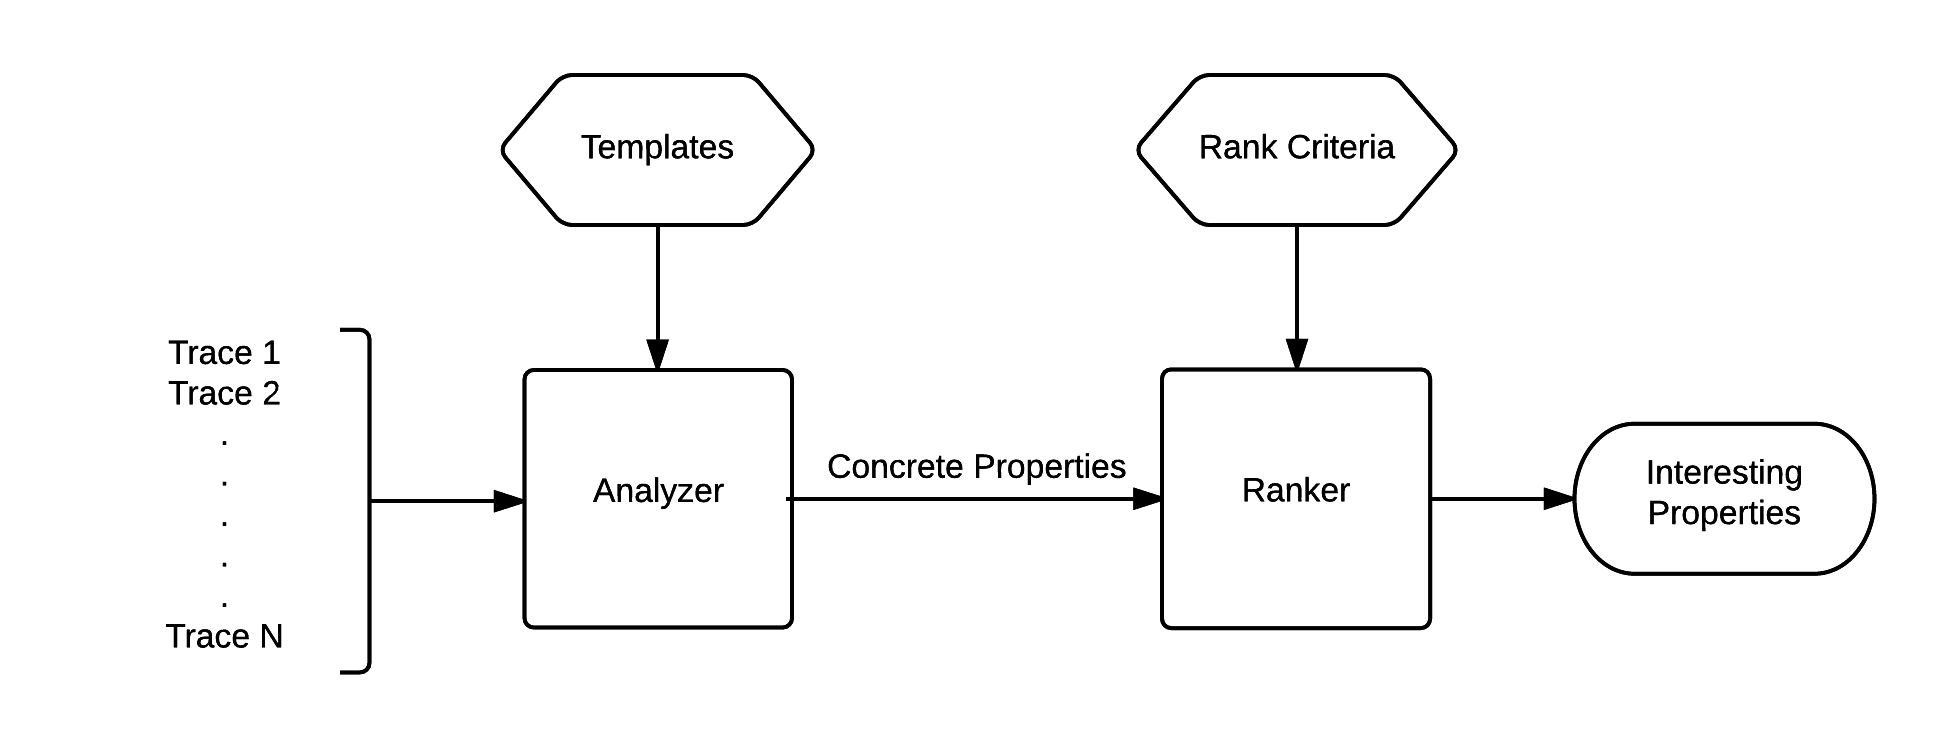
\includegraphics[trim = 1cm 0cm 0cm 0cm,clip = true,width=\linewidth]{figures/Workflow.png}
  \caption{Property Mining Workflow}
  \label{fig:work-flow Overview}
\end{figure}

\subsection{The Workflow}

We use traces of execution collected during the runtime of a system. The event traces are generated using instrumentation already present in the system and include network traffic logs, operating system logs, or program instrumentation logs. The analyzer accepts a set of N logs, where N $\ge$ 1.

The templates in Figure 1 refer to templates of temporal properties - timed regular expressions ~\cite{timedregex} that encode constraints on the relationships between subsets of trace events. Each template is an abstraction of the desired temporal property, like request, alternating, etc. ~\cite{evans1}. A template uses an abstract set of symbols ranging from 0 to L, where L is the length of the abstract alphabet. It also uses operators and time intervals as defined in ~\cite{timedregex}. For instance, (1.\textless0\textgreater[2,5])+ is a template for the response pattern. The '.' is the concatenation operator and the '+' is the operator for one or more instances of the expression.  The template specifies that some log event 1 is followed by another log event 0 within 2 to 5 time units, and this pattern occurs at least once in the execution trace. 

The abstract alphabet is used as a placeholder. The analyzer extracts a set of S unique event symbols from the collected traces and substitutes these in place of the abstract symbols to form concrete temporal properties. In the case of (1.\textless0\textgreater[2,5])+ the analyzer will evaluate the property for all combinations of two events in S. The key insight for achieving O(nL) time complexity is that an event X from the trace can be treated as either a P event or an S event.


Using an incidence matrix of dimension L we will evaluate which event combinations satisfy the given property. The acceptor FSM will iterate over the events in the system log and at each new event evaluate if any of the combinations in the matrix are satisfied. The matrix keeps track of the number of successes and failures to evaluate each concrete temporal property. 

\subsection{Dominant Properties}

The concrete properties examined by the analyzer contain every permutation of trace events within the template. These contain both interesting and frequently occurring patterns, as well as those that might have been found just a handful of times in the trace. Since the number of concrete properties could be very large, $S^L$, a ranking component is used to reduce the set to interesting properties only. 

The effectiveness of selecting a meaningful subset of properties depends on picking a good set of criteria and associated satisfaction thresholds. The ranking criterion we use is a combination of support and probability. Support is the percentage of all traces that contain the concrete property. Probability is the ration of successful evaluations of the property over total possible occurrences. We specify a threshold for these measures to extract properties that are consistently dominant in the collected traces. In section X our experiments explore the appropriate values for the thresholds.

Another motivation for using the ranker is the presence of imperfect traces. Traces can be imperfect as a result of dropped events or execution of faulty programs. In such cases, properties may not be perfectly satisfied in the collected traces. By using the probability and support ranking criteria we focus on finding the dominant properties in the trace. 


\section{Discussion}
%% author: GC

Our work mines temporal properties that can be expressed using timed regular expressions. The following discussion explores how the chosen approach accomplishes this and why it does so optimally.

\subsection{Using Timed Automata as Acceptors}

First we can look at regular expressions and their acceptors without the timing constraints. Regular expressions offer a declarative way to express the patterns that we want to accept. Every language defined by a regular expression is also defined by a finite automaton, as defined by Theorem 3.7 in ~\cite{book1}. There is a way to convert any regular expression into a non-deterministic automaton, and further to convert from a non-deterministic to a deterministic automaton. We can thus generate a Deterministic Finite Automaton (DFA) for any regular expression.

Similarly, timed automata are recognizers of timed languages. They have states, as any FSM, as well as clocks. Every timed language defined by a (generalized extended) regular expression is accepted by a timed automaton, as defined by Theorem 2 in ~\cite{timedregex}. Thus, timed automata and generalized timed regular expressions have the same expressive power. 

The language of a timed automaton consists of all the strings that it accepts ~\cite{timedregex}. The strings in our case are sequences of time-event pairs. The timed automata we generate are acceptors for strings that satisfy the desired property. The more strings in the trace that can be accepted, the more dominant is the property.

\subsection{Memory Requirements}

The main space requirement of our approach is for containing the matrix. The dimensionality L of the matrix depends on the number of abstract symbols in the desired property. The more events present in the relationship that the property encodes, the more dimensions of the matrix will be required. 

Each dimension of the matrix will consist of S unique event symbols. We want to encode the matrix to hold the evaluation results of every combinatorial combination of unique events. Thus we need $S^L$ space to hold acceptor results.

The number of unique events S in the trace will depend on the complexity of the program or system. However more concerning is the dimensionality since it will lead to exponential growth of the space requirements.

Majority of properties that people care about most represent relationships among a few events ~\cite{evans1, dwyer}. Thus the dimension L of the matrix will be constrained (How should we quantify that? Constrained to at most X events).

Since our approach examines one event from the trace at a time, trace storage does not need to be replicated.

The storage required for the FSM is proportional to the number of states. n is the length of the regular expression, then NFA has O(n) states and DFA has at most $O(S^n)$ states.

\subsubsection{CPU Requirements}

TBD

Length of a single trace T - the number of lines/entries of time-event combinations. 
The FSM will iterate over the trace once. At each trace line it will check the satisfiability for each entry in the matrix (All or just for the event it just read from the trace?). The overall runtime will this be $T * S^L$. 
This is a huge benefit as the length of traces can be huge, much larger than the complexity of the property. 
The processing complexity for each character in the input is O(1) in a DFA.
The key insight for achieving $O(ST)$ time complexity is that an event X from the trace can be treated as either a 0 event or a 1 event. (that was true in the peracotta paper for a property with 2 symbols only)

\subsubsection{Optimality}

TBD

Why finite state machines are fastest for checking satisfiability of property in a trace? 

Since the properties are contained in a regular language, we can efficiently analyze them. The efficient analysis applies to any property that falls into the regular language. Each one can be represented with a matrix. 

Why is using the matrix ensure fastest runtime?

\subsubsection{Scaling the Approach}

TBD

How does the algorithm scale with respect to the property that we mine?

The scalability of dynamic property mining techniques is generally limited.
The techniques scale poorly with the size of the input trace. 


The number of symbols present in the property directly influences the matrix size. Thus the more complex the property, the more memory space will be required to store the results. 

The automaton for the property is generated once at the start. The automaton is then reused for every cell in the matrix.

\section{Conclusion}

TBD


%\bibliographystyle{abbrv}
\bibliographystyle{plainnat}
\bibliography{refs}


\end{document}


